\chapter{Lecture 4 - Applied Perception}
As we have already seen, information visualization is about transforming data into visual representation so that a human can extract useful information out of it. The effectiveness of a visual representation is not arbitrary; it strongly depends on how brain works. That's why understanding how perception works can help one make informed decisions about visualization designs.

\begin{definition}[Contrast Sensitivity Function]
    Our perception is sensitive to pattern contrast frequency and orientation, also color influences the perception as well. 
\end{definition}

\begin{definition}[Perceptive field in retina]
    The perceptive field of a cell is the visual area over which a cell responds to light. Retinal ganglion cells are organized with circular receptive fields, which are stimulated on-center when excited and stimulated off-center when inhibited.
\end{definition}

\section{Grayscale maps}
The visual effects can result in large errors when reading quantitative information maps displayed using a grayscale map --> use grayscale maps to represent a few values, and not to map or to compare many values.\par
It is useful for highlighting or show boundaries, important items by reducing contrast of unimportant ones; or to adjust background luminance to obtain better readability.

\subsection{Cornsweet illusion}
The lateral inhibition can be considered part of an edge detection process in a scene under viewing. Pseudo-edges can be seen depending on the stimulus.\par
The brain does perceptual interpolation so that regions affected by such edges can appear lighter or darker. This is called \emph{Cornsweet illusion}. 
\begin{figure}[thbp]
    \centering
    
\includegraphics[width=0.4\linewidth]{imgs/lecture4/4.1 cornsweet illusion.png}
    \caption{The Cornsweet effect}
    \label{fig:4.1}
\end{figure}

In the fig~\ref{fig:4.1}, an example of the Cornsweet effect shows the separating line between the shades of gray.

\section{Eye movement}
\begin{itemize}[noitemsep]
    \item \emph{Saccadic} movement: \emph{ballistic} movements of the eyes that change the point of fixation. They can be voluntary or stimulus-elicited
    \item \emph{Smooth-pursuit} movement: \emph{slow tracking} movements of the eyes to keep a moving stimulus on the fovea (a nerve in the eye)
    \item \emph{Vergence} movement: align the fovea of each eye to a target according to its distance
    \item \emph{Vestibulo-ocular} movement: \emph{stabilize} the eyes compensating for head movements
\end{itemize}

\subsection{Saccadic movement and fixations}
The Saccadic eye movements take between 20 to 180 ms. It makes both eyes move in the same direction. This movement may not be a simple linear trajectory.

\begin{definition}[Fixation]
    A fixation is composed of slower and finer movements (microsaccades, tremors, and drift) that help the eye align with the target. A fixation varies between 50 and 600 ms.
\end{definition}

For instance, a typical movement of this kind during reading moves the eyes for 2 degrees, and in general, the movement is between 2 and 5 degrees. If the movement is larger than 20 degrees, the head movement is required.

\section{Pre-attentive process}
Some visual stimuli naturally "pop up" from their surroundings, especially when all the items are of the same characteristics except for one. These "pop-up" features can be: orientation, curvature, shape, size, color, light/dark, enclosure, concavity/convexity, or addition. 

\begin{figure}[htbp]
    \centering

    \begin{subfigure}[b]{0.32\linewidth}
        \centering
        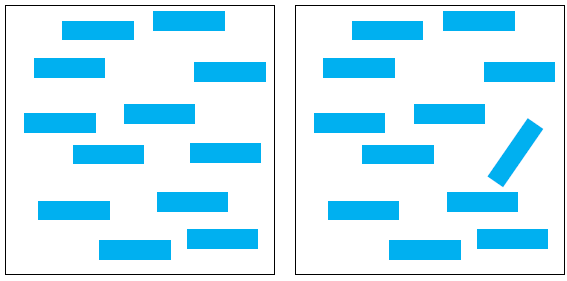
\includegraphics[width=\linewidth]{imgs/lecture4/4.2 preattentive-orientation.png}
        \caption{orientation}
        \label{fig:4.2a}
    \end{subfigure}
    \hfill
    \begin{subfigure}[b]{0.32\linewidth}
        \centering
        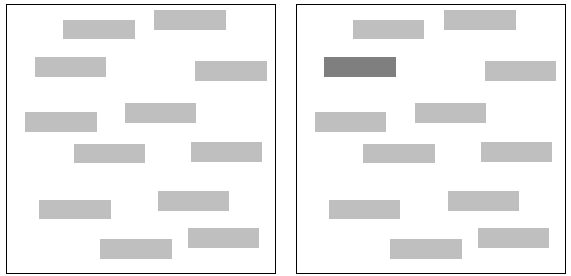
\includegraphics[width=\linewidth]{imgs/lecture4/4.3 preattentive-light dark.png}
        \caption{Light/Dark}
        \label{fig:4.2b}
    \end{subfigure}
    \hfill
    \begin{subfigure}[b]{0.32\linewidth}
        \centering
        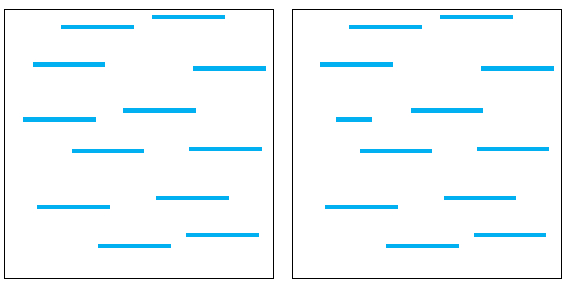
\includegraphics[width=\linewidth]{imgs/lecture4/4.4 preattentive-length.png}
        \caption{Length}
        \label{fig:4.2c}
    \end{subfigure}

    \caption{Features that pop up}
    \label{fig:4.2}
\end{figure}

In the fig~\ref{fig:4.2}, some examples of how some visual features are pre-attentively processed.

\subsection{Asymmetry}
Some pre-attentive processes are not symmetric.
\begin{itemize}[noitemsep]
    \item Adding marks is more efficient than removing marks
    \item Increasing sharpness is more efficient than decreasing sharpness
    \item A big object surrounded by small objects is more efficient than the other way around
\end{itemize}

\begin{figure}[htbp]
    \centering

    \begin{subfigure}[b]{0.32\linewidth}
        \centering
        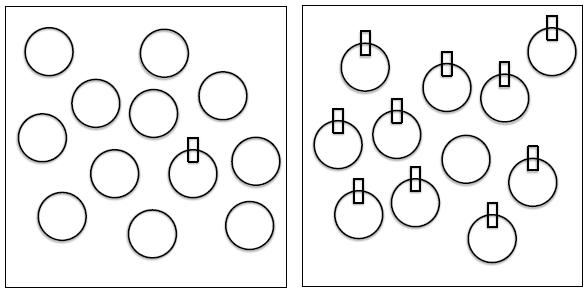
\includegraphics[width=\linewidth]{imgs/lecture4/4.5 asymmetry-marsk.png}
        \caption{Marks}
        \label{fig:4.3a}
    \end{subfigure}
    \hfill
    \begin{subfigure}[b]{0.32\linewidth}
        \centering
        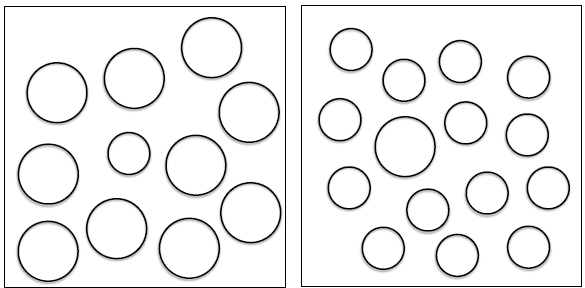
\includegraphics[width=\linewidth]{imgs/lecture4/4.6 asymmetry-size.png}
        \caption{Size}
        \label{fig:4.3b}
    \end{subfigure}
    \hfill
    \begin{subfigure}[b]{0.32\linewidth}
        \centering
        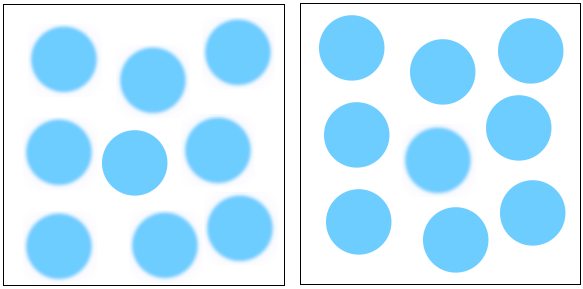
\includegraphics[width=\linewidth]{imgs/lecture4/4.7 asymmetry-sharpness.png}
        \caption{Sharpness}
        \label{fig:4.3c}
    \end{subfigure}

    \caption{Asymmetry of pre-attentive process}
    \label{fig:4.3}
\end{figure}

In the fig~\ref{fig:4.3}, some examples of how some of the asymmetry of the pre-attentive process works. For instance, an object with an additional mark is much more noticeable than an object without a mark.\par

\subsection{Feature combination}
Note that different combinations of pre-attentive visual features may not be pre-attentive.

In the fig~\ref{fig:4.4} shows an example of combining shape and color visual features in an attempt to obtain the "pop up" effect, but the actual result is not as good as we thought.
\begin{figure}[htbp]
    \centering
    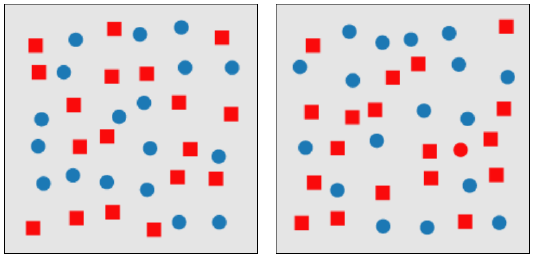
\includegraphics[width=0.4\linewidth]{imgs/lecture4/4.8 preattentive combinations.png}
    \caption{Where is the red circle?}
    \label{fig:4.4}
\end{figure}

\section{Gestalt laws}
It is an attempt to understand pattern perception. It is a powerful ally in visual perception, for example, to show group elements, to show relationships, to make pattern comparisons, in an effective way:
\begin{itemize}[noitemsep]
    \item Proximity: objects close to each other are perceived to form a group
    \item Similarity: similar objects are perceived to form a group
    \item Connectedness: connected objects are perceived as related; most of the time, connecting different objects with a line is a powerful way to express a relationship between the objects.
    \item Continuity: we expect that a line or an edge continues to follow its direction and does not deviate from it
    \item Symmetry: objects arranged symmetrically are perceived as forming a visual whole instead of being perceived as separate entities
    \item Closure: we tend to perceive the complete appearance of an object so that our brain fills the gap in case of missing parts
    \item Common fate: we tend to perceive a group of object that moves in the same direction as a whole
    \item Figure-ground: the perceptual effect regards the formation of a figure from the background
\end{itemize}

\begin{figure}[htbp]
    \centering

    \begin{subfigure}[b]{0.32\linewidth}
        \centering
        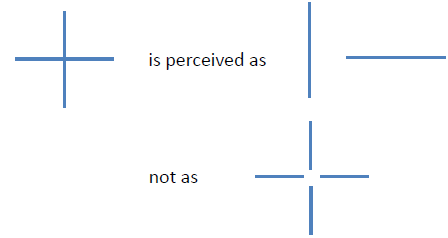
\includegraphics[width=\linewidth]{imgs/lecture4/4.9 connectedness.png}
        \caption{Connectedness}
        \label{fig:4.5a}
    \end{subfigure}
    \hfill
    \begin{subfigure}[b]{0.32\linewidth}
        \centering
        
\includegraphics[width=0.5\linewidth]{imgs/lecture4/4.10 closure.png}
        \caption{Closure}
        \label{fig:4.5b}
    \end{subfigure}
    \hfill
    \begin{subfigure}[b]{0.32\linewidth}
        \centering
        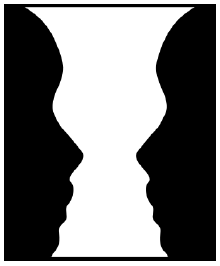
\includegraphics[width=0.5\linewidth]{imgs/lecture4/4.11 figure ground.png}
        \caption{Figure-ground}
        \label{fig:4.5c}
    \end{subfigure}

    \caption{Gestal laws examples}
    \label{fig:4.5}
\end{figure}